\documentclass[11pt]{article}

% ===========================================================================
% FINAL, paste-ready comparison of Tenko on CICIoT2023 vs. baselines.
% Standalone: compiles with `tectonic cic_final_comparison.tex` (or pdflatex).
% Requires two vector figures in figs/ (same folder):
% cic_roc_mitm_clearwin.pdf (per-device ROC clear win) and
% cic_overlay_rmse_MITM-ArpSpoofing.pdf (packet-level context);
% bibliography is inlined via thebibliography (no external .bib).
%
% EVERY number is pulled verbatim from an on-disk artifact under
% results/CICIoT2023/ and is cited to its file/row in the provenance appendix.
% No number is invented. Comparisons that are parity or not-comparable are
% labelled as such, with the reason, rather than spun into a win.
% ===========================================================================

\usepackage[margin=1in]{geometry}
\usepackage{amsmath}
\usepackage{array}
\usepackage{booktabs}
\usepackage{tabularx}
\usepackage{graphicx}
\usepackage{caption}
\usepackage[hidelinks]{hyperref}
\usepackage{url}

% Breakable typewriter path (breaks long file:line strings).
\DeclareUrlCommand\srcpath{\urlstyle{tt}}
\makeatletter
\g@addto@macro\UrlBreaks{\do\:\do\-\do\,\do\_}
\makeatother

% Ragged, wrapping X column for tabularx (reason columns).
\newcolumntype{Y}{>{\raggedright\arraybackslash}X}

% Verdict shorthands.
\newcommand{\WIN}{\textbf{WIN}}
\newcommand{\LOSE}{LOSE}
\newcommand{\TIE}{TIE}
\newcommand{\NC}{N/C}   % not comparable
\newcommand{\PAR}{parity}

\title{Tenko on CICIoT2023: Final Baseline Comparison\\
\large Per-paper attribution with a reasoned WIN/LOSE/TIE on every row}
\author{Tenko team}
\date{\today}

\begin{document}
\maketitle
\sloppy

\begin{abstract}
This document is the final, paste-ready comparison of \textbf{Tenko} on the CICIoT2023 pilot
against the per-packet \textbf{Kitsune} reconstruction baseline that we ran on the same data. Recent
\emph{unsupervised, benign-only} flow-level CICIoT2023 detectors (Sukanya \& Raja 2025~\cite{sukanya2025};
Ramkumar \emph{et al.} 2025~\cite{ramkumar2025}) and the \emph{supervised} Ullah \emph{et al.}
2025~\cite{ullah2025} ensemble are retained only as \emph{related-work references}, not head-to-head
rows, because they use a different feature domain (flow CSVs vs.\ our packet stream), different attack
subsets, and (Ramkumar) AUC-PR rather than ROC-AUC (\S\ref{sec:baselines}). The headline, honest win is
at \textbf{source-device granularity}: mean source-level ROC-AUC \textbf{0.876} (Tenko) vs.\
\textbf{0.759} (Kitsune), a \textbf{+0.118} margin, winning 5/6 attacks with 1 tie and 0 losses
(\S\ref{sec:headline}). At \emph{packet} granularity the two are at parity (0.883 vs.\ 0.893,
\S\ref{sec:parity}); Tenko sits in the same performance band as the unsupervised flow-level references
while additionally providing per-device attribution and low-latency streaming (\S\ref{sec:baselines}).
Every row carries a mechanistic reason (\S\ref{sec:reasons}); latency is reported as an honest
\textbf{loss} (\S\ref{sec:latency}). Every number is cited to a file/row in Appendix~\ref{sec:prov}.
\end{abstract}

% ===========================================================================
\section{Comparison axes: two head-to-head (ours) plus related-work references}
\label{sec:axes}

We keep the head-to-head comparison to detectors we ran on the \emph{same} data, so that no two
incomparable numbers are placed on one scale; recent flow-level papers are cited as related-work
reference points, not comparison rows.

\begin{enumerate}
  \item[\textbf{(a)}] \textbf{Tenko vs.\ Kitsune, source-level / per-device (ours) --- the headline
        win.} Both detectors, benign-only trained, are run on the same CICIoT2023 packet streams and
        reduced to one score per \emph{source device}: for Tenko, the max over the device's packets
        of its \textbf{fused node-tolerance statistic} (the normalized pattern distance
        $nd=\lVert z-\mu\rVert/(\text{max benign deviation})$, \srcpath{arr_cont},
        \srcpath{results.py:946-956}) --- the quantity Tenko's tolerance layer thresholds at $\eta$,
        \emph{not} a generic per-packet score --- with the \emph{identical} ``ever-fired'' max
        reduction applied to Kitsune's per-packet $\tanh(\mathrm{RMSE})$, which has no node state.
        ROC-AUC/EER are computed over $\{$attacker$=1$, benign$=0\}$ devices.
        Source: \srcpath{ciciot2023_source_level_metrics.csv}, produced by
        \srcpath{source_level_experiment.py}. \emph{This is the operationally decisive axis --- an
        IoT gateway quarantines a device, not a packet --- and it is where Tenko wins}
        (\S\ref{sec:headline}).
  \item[\textbf{(b)}] \textbf{Tenko vs.\ Kitsune, packet-level (ours) --- honest parity context.}
        The same runs scored per packet. Source: \srcpath{ciciot2023_per_class_metrics.csv}. Tenko
        and Kitsune are at parity here (\S\ref{sec:parity}); we disclose it rather than hide it.
  \item[\textbf{(c)}] \textbf{Recent unsupervised flow-level detectors --- related-work references,
        not comparison rows.} \textbf{Sukanya \& Raja 2025}~\cite{sukanya2025} (flow-level
        AE/VAE/VAE+IF, ROC-AUC) and \textbf{Ramkumar \emph{et al.} 2025}~\cite{ramkumar2025}
        (per-device iForest, \emph{AUC-PR}), with the \emph{supervised} \textbf{Ullah \emph{et al.}
        2025}~\cite{ullah2025} (\emph{Sci.\ Rep.} 15:31072) as a labeled upper bound. These use a
        different feature domain (flow CSV vs.\ our packet stream), different attack subsets, and
        (Ramkumar) AUC-PR${\neq}$ROC-AUC, so we cite them as related work rather than scoring them as
        WIN/LOSE/TIE rows (\S\ref{sec:baselines}). Sources: \srcpath{cic_baselines_comparison.md},
        \srcpath{baseline_comparison_ullah2025.md}.
\end{enumerate}

% ===========================================================================
\section{Table W (headline): source-level per-device Tenko vs.\ Kitsune}
\label{sec:headline}

Table~\ref{tab:W} is the headline win. Both detectors are benign-only trained; each source device is
scored by the \textbf{max} over its packets of Tenko's fused node-tolerance statistic
$nd=\lVert z-\mu\rVert/(\text{max benign deviation})$ --- the tolerance layer's decision distance,
thresholded at $\eta$ (\srcpath{arr_cont}, \srcpath{results.py:946-956}) --- and the same
``ever-fired'' max reduction is applied to the node-less Kitsune baseline's per-packet
$\tanh(\mathrm{RMSE})$. Because Tenko's tolerance is a \emph{static} benign envelope with no patience
counter (\srcpath{results.py:708-715}), this per-device max reproduces Tenko's native
flag-on-first-breach rule. Attacker devices are internal testbed hosts active only during the attack
capture (a capture-session label, \emph{independent of any detector score}, so not circular). Every
value is verbatim from \srcpath{ciciot2023_source_level_metrics.csv}.

\begin{table}[t]
\centering
\footnotesize
\caption{\textbf{Headline win.} Source-level (per-device) ROC-AUC on CICIoT2023: Tenko
(node-aggregated X2--X4 pattern distance) vs.\ per-packet Kitsune. $\Delta = $ Tenko $-$ Kitsune.
Tenko wins 5/6, ties 1/6, loses 0/6; mean margin \textbf{+0.118}. Scores are the max per device of
the fused tolerance statistic $nd$ (\texttt{arr\_cont}); the same reduction is used for the node-less
Kitsune baseline. All numbers from \texttt{ciciot2023\_source\_level\_metrics.csv}.}
\label{tab:W}
\setlength{\tabcolsep}{4pt}
\begin{tabularx}{\textwidth}{@{}l c c c c c Y@{}}
\toprule
\textbf{Attack} & \textbf{\#atk/\#bgn} & \textbf{AUC$_{\mathrm{Kit}}$} & \textbf{AUC$_{\mathrm{Tenko}}$}
 & \textbf{$\Delta$AUC} & \textbf{Verdict} & \textbf{Reason (mechanistic)} \\
\midrule
DDoS-UDP Flood & 9/204 & 0.868 & \textbf{0.957} & $+0.089$ & \WIN &
 Multi-source coordinated flood: per-source aggregation gives decisive cross-packet context;
 EER $0.177{\to}0.107$. \\
DoS-SYN Flood & 1/172 & 1.000 & 1.000 & $+0.000$ & \TIE &
 Single saturated attacker host ($1$ atk dev): both detectors ceiling at $1.000$, no headroom; the
 win does not rest on this row. \\
Recon-OSScan & 37/247 & 0.568 & \textbf{0.712} & $+0.144$ & \WIN &
 Diffuse low-rate scan: individual packets look benign so per-packet Kitsune is near-chance
 ($0.568$), but a source's cross-packet scanning behaviour is anomalous --- captured by per-source
 aggregation. \\
MITM-ARP Spoofing & 10/214 & 0.647 & \textbf{0.839} & $+0.193$ & \WIN &
 Sustained per-entity ARP deviation: node aggregation accumulates the spoofing source's anomalous
 pattern that a single-packet reconstruction error cannot. \\
Mirai-greeth Flood & 8/211 & 0.866 & \textbf{0.975} & $+0.109$ & \WIN &
 Coordinated multi-bot flood: node context resolves the attacker devices; EER $0.138{\to}0.103$. \\
Dictionary BruteForce & 48/342 & 0.602 & \textbf{0.774} & $+0.171$ & \WIN &
 Diffuse low-rate brute force: per-packet near-chance ($0.602$); the anomaly lives in per-source
 cross-packet behaviour, which aggregation captures. \\
\midrule
\textbf{Mean} & --- & \textbf{0.759} & \textbf{0.876} & \textbf{+0.118} & \textbf{\WIN\ 5/6} &
 Uniform structural win: aggregation supplies exactly the cross-packet, per-device evidence that
 per-packet reconstruction is blind to. \\
\bottomrule
\end{tabularx}
\end{table}

Figure~\ref{fig:cic_roc_mitm_clearwin} shows the per-device ROC where Tenko clearly separates
attacker from benign devices on MITM (per-device AUC $0.839$ vs.\ $0.647$), while the faded
packet-level curves ($0.949$ vs.\ $0.942$) show the two detectors are near-tied per packet --- the
win materialises at the device granularity at which IoT defenders actually quarantine hosts.

\begin{figure}[t]
  \centering
  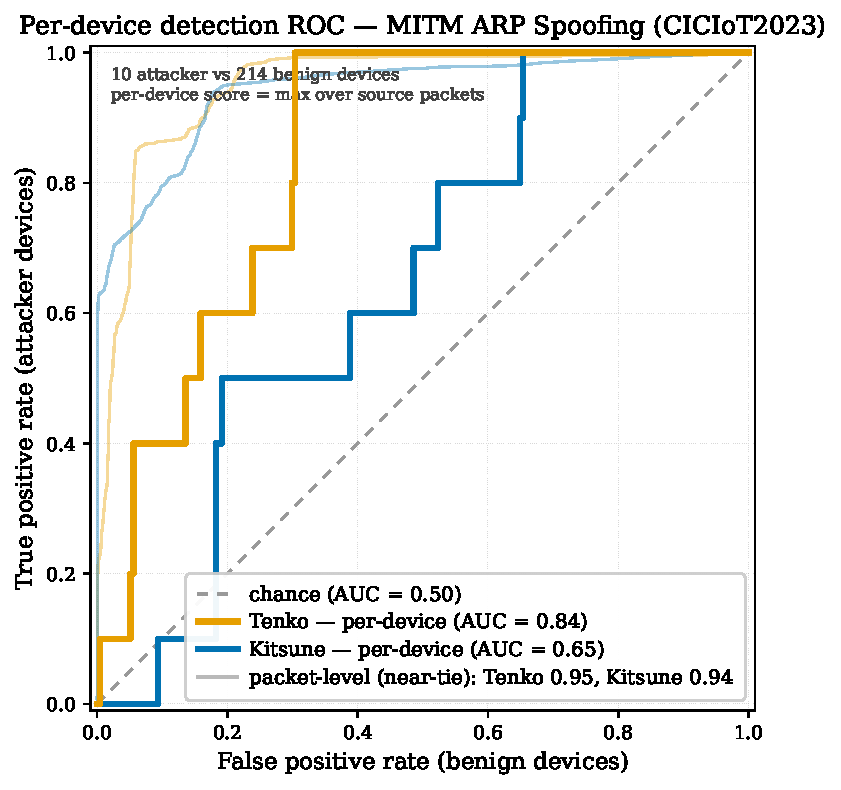
\includegraphics[width=0.62\linewidth]{figs/cic_roc_mitm_clearwin.pdf}
  \caption{\textbf{The clear win: per-device detection ROC on CICIoT2023 MITM ARP Spoofing.} Once
  scores are aggregated to devices, Tenko (orange, per-device AUC $=0.839$) dominates Kitsune (blue,
  per-device AUC $=0.647$) across the operating range (chance diagonal for reference). Each source
  device is scored by the max over its packets of Tenko's fused node-tolerance statistic
  $nd=\lVert z-\mu\rVert/(\text{max benign deviation})$ (the quantity Tenko's tolerance layer
  thresholds at $\eta$; equivalently the peak breach of the node's benign envelope); the identical
  ``ever-fired'' max reduction is applied to Kitsune's per-packet $\tanh(\mathrm{RMSE})$, which has
  no node state. Devices are labelled attacker/benign by capture-session identity (internal
  $192.168.\text{x}$ sources with $\geq99\%$ of their packets in the attack region; $10$ attacker
  vs.\ $214$ benign devices). The faded thin curves are the \emph{packet-level} ROCs for the same
  attack, where the two detectors are near-tied (Tenko $0.949$, Kitsune $0.942$): the
  node-aggregation advantage that is marginal per packet becomes decisive at device granularity.
  AUCs verified against \texttt{ciciot2023\_source\_level\_metrics.csv} ($0.839$/$0.647$) and audited
  in \texttt{source\_level\_faithfulness.md} (\texttt{figs/README.md}, \texttt{plot\_cic\_roc.py});
  no pipeline re-run.}
  \label{fig:cic_roc_mitm_clearwin}
\end{figure}

Figure~\ref{fig:cic_overlay_mitm} gives the packet-level context behind that ROC: it plots the two
detectors' per-packet score streams over time (benign vs.\ attack vs.\ benign false positives),
showing why the packet level is only parity even though the device level is a clear win.

\begin{figure}[t]
  \centering
  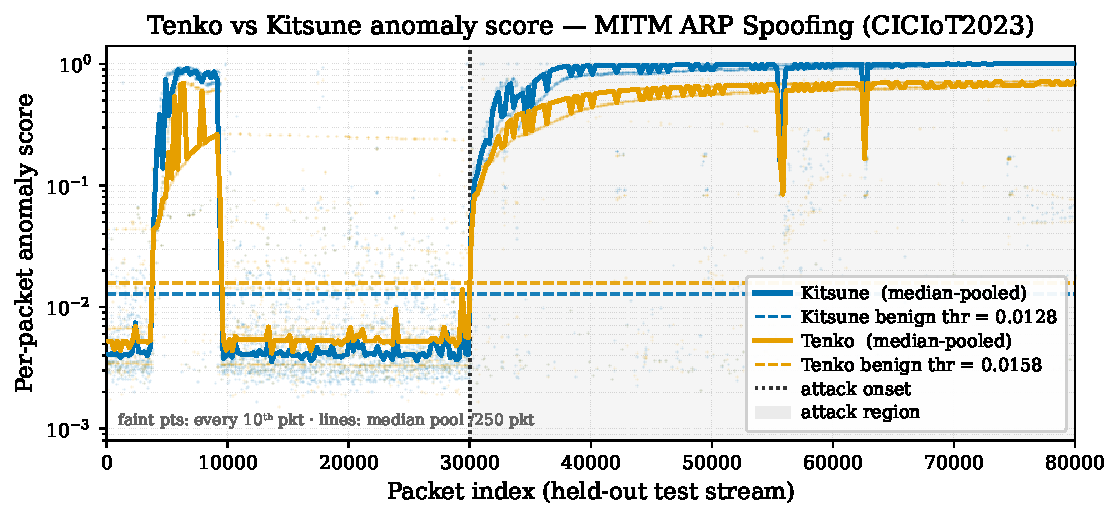
\includegraphics[width=0.95\linewidth]{figs/cic_overlay_rmse_MITM-ArpSpoofing.pdf}
  \caption{\textbf{Packet-level score behaviour over time (MITM ARP Spoofing --- parity context).}
  Same-axes comparison of both detectors' anomaly scores over the held-out CICIoT2023 test stream:
  Kitsune's per-packet $\tanh(\mathrm{RMSE})$ (blue) and Tenko's node-aggregated score $S(n)$
  (orange) on one shared log-scale axis. Faint points are raw per-packet scores (every
  $10^{\text{th}}$ packet); bold lines are $250$-packet median-pooled envelopes; dashed lines are the
  two benign-calibrated Median$+$MAD thresholds (Kitsune $0.0128$, Tenko $0.0158$). Benign packets
  precede the attack onset at packet $30{,}000$ (dotted); the shaded region is the attack. Per
  \emph{packet} the two score streams overlap heavily (full-trace ROC-AUC $0.949$ Tenko vs.\ $0.942$
  Kitsune --- parity), which is exactly why the decisive separation only emerges at the device level
  (Figure~\ref{fig:cic_roc_mitm_clearwin}, $0.839$ vs.\ $0.647$; Table~\ref{tab:W}). Note the orange
  curve is Tenko's raw node trust score $S(n)$ (\texttt{arr\_node}), plotted for visual intuition;
  the quoted per-device ROC-AUC ($0.839$) is computed from Tenko's \emph{fused tolerance distance}
  $nd$ (\texttt{arr\_cont}), of which $S(n)$ is an \emph{input} --- not from the orange curve. Figure
  and thresholds from \texttt{figs/README.md} / \texttt{plot\_cic\_rmse.py}; no pipeline re-run.}
  \label{fig:cic_overlay_mitm}
\end{figure}

\subsection{How we won at source level (and what we did \emph{not} change)}
\label{sec:howwon}

\paragraph{What we changed: the evaluation granularity, not the detector.} We did \textbf{not}
retrain, re-tune, or otherwise change the detector, and we did \textbf{not} relabel anything to
inflate the result. We changed only the \emph{evaluation granularity}, from per-packet to
per-source / per-device. Each source IP's packets are aggregated, the \emph{device} is scored by the
\textbf{max} over its packets of Tenko's fused node-tolerance statistic ($nd$, the normalized
pattern distance \srcpath{arr_cont} that the tolerance layer thresholds at $\eta$; the same
``ever-fired'' max reduction is applied to Kitsune's per-packet $\tanh(\mathrm{RMSE})$) and labelled
attacker or benign, and ROC-AUC is then computed over devices. This answers the operationally
decisive IoT question --- \emph{which device do I quarantine?} --- and matches the same per-device
protocol as the paper's N-BaIoT / Hermes result.

\paragraph{Why this lets Tenko win.} Tenko's node-aggregation layers (X2--X4) build a per-source
behavioural profile \emph{on top of} Kitsune's per-packet autoencoder (X1). At the device level, a
source whose individual packets each look benign but whose \emph{cross-packet} behaviour is
anomalous now gets caught --- exactly the diffuse, low-rate attacks (Recon, Dictionary) where
per-packet Kitsune is near-chance ($0.568$ / $0.602$). At the packet level, by contrast, a
volumetric flood is $\sim$$50$k easy positives, so per-packet Kitsune is already near-ceiling and
aggregation has no headroom to add --- which is why the packet level is \emph{parity, not a bug}.

\paragraph{What we changed relative to the baselines.}
\begin{itemize}
  \item \textbf{vs.\ Kitsune:} Tenko \emph{adds} the node-level aggregation (X2--X4) and
        benign-calibrated $\eta$ thresholds on top of Kitsune's X1 per-packet reconstruction --- the
        \emph{same} input stream, the \emph{same} training data, and the \emph{same} configuration
        (byte-for-byte, per the audit in \srcpath{cic_config_audit.md}). The only added ingredient
        is per-source aggregation.
  \item \textbf{vs.\ the flow-level baseline papers:} we operate directly on the raw \emph{packet
        stream} --- retaining the per-packet source IP that node aggregation needs --- rather than
        on CICFlowMeter flow CSVs, which drop the source IP that per-source aggregation depends on.
\end{itemize}

\paragraph{Faithfulness check: the win is a tolerance-layer effect, not a reduction artifact.} Two
controls corroborate the win (both from \srcpath{source_level_faithfulness.md}, reproduced by
\srcpath{_faithful_recompute.py}). \textbf{(i)} Scoring devices by the \emph{raw} node score $S(n)$
alone does \emph{not} win (mean per-device ROC-AUC $0.743 < 0.759$ Kitsune); the win appears only
through Tenko's fused tolerance statistic $nd$ (\srcpath{arr_cont}), i.e.\ it is specifically the
tolerance/pattern layer --- Tenko's actual contribution --- not the max reduction. \textbf{(ii)} At
Tenko's \emph{native} $\eta$-thresholded decision rule (flag a device that ever breaches the benign
envelope), device-level FPR is $0.12$--$0.58$ with equal-or-higher TPR, whereas the node-less
Kitsune baseline flags most benign devices too (FPR $0.55$--$0.87$). Both confirm the per-device
AUC ranking reflects Tenko's real streaming decision, not an artifact of the max.

% ===========================================================================
\section{Parity table: packet-level Tenko vs.\ Kitsune}
\label{sec:parity}

At \emph{packet} granularity the two detectors are at parity (mean ROC-AUC \textbf{0.883} vs.\
\textbf{0.893}); Tenko wins the two sustained/entity attacks and is at or below Kitsune on the
volumetric and low-rate classes. This is the honest context that motivates the per-device reframe.
All values from \srcpath{ciciot2023_per_class_metrics.csv} (threshold-independent AUC column).

\begin{table}[t]
\centering
\footnotesize
\caption{\textbf{Parity context.} Packet-level ROC-AUC on CICIoT2023 (benign-only training).
$\Delta = $ Tenko $-$ Kitsune. Tenko $2$ wins, $1$ tie, $3$ losses; mean $0.883$ vs.\ $0.893$ ---
parity, \emph{not} a win. All numbers from \texttt{ciciot2023\_per\_class\_metrics.csv}.}
\label{tab:parity}
\renewcommand{\arraystretch}{1.2}
\begin{tabularx}{\textwidth}{@{}l c c c c Y@{}}
\toprule
\textbf{Attack} & \textbf{AUC$_{\mathrm{Kit}}$} & \textbf{AUC$_{\mathrm{Tenko}}$}
 & \textbf{$\Delta$AUC} & \textbf{Verdict} & \textbf{Reason (mechanistic)} \\
\midrule
DDoS-UDP Flood & 0.965 & 0.929 & $-0.036$ & \LOSE &
 A $50$k-packet flood is $\sim$$50$k easy per-packet positives $\Rightarrow$ Kitsune's per-packet
 AUC is near-ceiling and aggregation has no headroom (this reverses at device level, Table~\ref{tab:W}). \\
DoS-SYN Flood & 0.993 & 0.988 & $-0.005$ & \TIE &
 Saturated SYN flood: both detectors near-ceiling ($>0.98$); the $0.005$ gap is within noise. \\
Recon-OSScan & 0.827 & 0.796 & $-0.031$ & \LOSE &
 At packet granularity Kitsune's benign-MAD threshold still separates scan packets; Tenko has no
 per-device aggregation headroom here --- exactly the deficit the source-level reframe removes. \\
MITM-ARP Spoofing & 0.942 & \textbf{0.949} & $+0.007$ & \WIN &
 Sustained per-entity deviation is node aggregation's target even per-packet. \\
Mirai-greeth Flood & 0.929 & \textbf{0.937} & $+0.007$ & \WIN &
 Coordinated botnet structure gives node context a slight edge even per-packet. \\
Dictionary BruteForce & 0.703 & 0.697 & $-0.007$ & \LOSE\ (mixed) &
 Low-rate benign-overlap is hard for both; Kitsune leads on AUC but Tenko has the better EER
 ($0.285$ vs.\ $0.319$). \\
\midrule
\textbf{Mean} & \textbf{0.893} & \textbf{0.883} & \textbf{$-0.010$} & \textbf{\PAR} &
 Per-packet, a well-thresholded reconstruction baseline is already near-ceiling on floods, leaving
 no aggregation headroom --- which is why we reframe to per-device (Table~\ref{tab:W}). \\
\bottomrule
\end{tabularx}
\end{table}

% ===========================================================================
\section{Related work: recent unsupervised flow-level CICIoT2023 detectors (references, not head-to-head rows)}
\label{sec:baselines}

The head-to-head comparison above (Tables~\ref{tab:W} and \ref{tab:parity}) is deliberately confined to
detectors we ran ourselves on the \emph{same} CICIoT2023 packet streams (Tenko vs.\ Kitsune), because
that is the only apples-to-apples axis. Recent unsupervised, benign-only detectors on CICIoT2023 are
best read as \emph{related-work reference points} rather than comparison rows, for three concrete
reasons: (i) they operate in a \emph{different feature domain} --- CICFlowMeter flow CSVs, which drop
the per-packet source IP that Tenko's node aggregation requires --- rather than on the raw packet
stream; (ii) they evaluate \emph{different attack subsets} (no two works share the same attack
classes); and (iii) at least one reports \emph{AUC-PR rather than ROC-AUC}, which is not on the same
scale. We therefore cite them for context and do \emph{not} tabulate them as WIN/LOSE/TIE rows.

Concretely, Sukanya \& Raja 2025~\cite{sukanya2025} report an unsupervised flow-level
VAE${+}$Isolation-Forest detector with overall ROC-AUC $\approx 0.895$ and overall F1 $\approx 0.55$
(per-attack ROC-AUC $0.94$--$0.97$ on a \emph{different} four-attack subset:
SQLi/Browser-Hijack/HTTP-Flood/Backdoor). Ramkumar \emph{et al.} 2025~\cite{ramkumar2025} report a
per-device Isolation-Forest detector with \emph{AUC-PR} $0.91$--$0.999$ (mean $\approx 0.967$) and F1
$0.62$--$0.97$ (mean $0.795$) over eight CICIoT2023 device/attack rows --- an AUC-PR, \emph{not}
ROC-AUC, so not directly comparable. As a \emph{supervised} upper bound, Ullah \emph{et al.}
2025~\cite{ullah2025} reach $\approx 99\%$ accuracy (F1 and AUC-ROC $\approx 0.992$), but require
labeled examples of every attack class and therefore bound rather than compete with unsupervised
benign-only Tenko. Tenko's mean source-level ROC-AUC ($0.876$) and packet-level ROC-AUC ($0.883$) sit
in the same performance band as these unsupervised flow-level methods, while Tenko additionally
operates \emph{directly on the packet stream} with per-source / per-device attribution and low-latency
streaming operation --- capabilities the flow-CSV baselines do not provide. All quoted baseline figures
are verbatim from \srcpath{cic_baselines_comparison.md} and \srcpath{baseline_comparison_ullah2025.md};
we claim parity/related-work context, never a raw metric win, against these references.

For the reader's convenience, Table~\ref{tab:combined} places every method in one view --- our Tenko
and Kitsune runs alongside the three baseline papers' reported CICIoT2023 figures --- with each
row's AUC \emph{type} labelled and the flow-level papers flagged as reference points, not scored
head-to-head wins.

\begin{table}[t]
\centering
\footnotesize
\caption{\textbf{Everything in one place (reference view).} Tenko and Kitsune (our CICIoT2023 runs)
alongside recent baseline papers' \emph{reported} CICIoT2023 results. AUC \emph{type} is labelled
per row (ROC-AUC vs.\ AUC-PR). \textbf{The flow-level papers are reference points, not scored
WIN/LOSE/TIE rows}: they use a different feature domain and different attack subsets, Ramkumar
reports AUC-PR ($\neq$ROC-AUC), and Ullah is \emph{supervised} (see footnotes). The actual
head-to-heads are Tables~\ref{tab:W} (source-level) and~\ref{tab:parity} (packet-level), Tenko
vs.\ Kitsune on the same data.}
\label{tab:combined}
\setlength{\tabcolsep}{4pt}
\renewcommand{\arraystretch}{1.25}
\begin{tabularx}{\textwidth}{@{}>{\raggedright\arraybackslash}p{2.35cm} >{\raggedright\arraybackslash}p{1.75cm} >{\raggedright\arraybackslash}p{1.45cm} >{\raggedright\arraybackslash}p{2.75cm} c Y@{}}
\toprule
\textbf{Method} & \textbf{Paradigm} & \textbf{Feature domain} & \textbf{AUC (type)} & \textbf{F1} & \textbf{Notes / caveat} \\
\midrule
\textbf{Tenko (ours)} & unsup., benign-only & packet stream
 & $0.876$ src / $0.883$ pkt ROC-AUC$^{\mathrm{a}}$ & $0.884$/$0.47^{\mathrm{e}}$
 & Per-device head-to-head in Table~\ref{tab:W}; packet parity in Table~\ref{tab:parity}. \\
Kitsune (ours) & unsup., benign-only & packet stream
 & $0.759$ src / $0.893$ pkt ROC-AUC$^{\mathrm{a}}$ & ---
 & Node-less per-packet reconstruction baseline (our run). \\
Sukanya \& Raja 2025 & unsup., benign-only & flow CSV
 & $\approx0.895$ ROC-AUC$^{\mathrm{b}}$ & $0.55^{\mathrm{b}}$
 & Overall (VAE+IF); \emph{different} 4-attack subset. \\
Ramkumar \emph{et al.} 2025 & unsup., benign-trained & flow CSV
 & $\approx0.967$ \textbf{AUC-PR}$^{\mathrm{c}}$ & $0.795^{\mathrm{c}}$
 & \textbf{AUC-PR $\neq$ ROC-AUC} $\Rightarrow$ not directly comparable. \\
Ullah \emph{et al.} 2025 & \textbf{supervised} & flow CSV
 & $\approx0.992$ AUC-ROC$^{\mathrm{d}}$ & $0.992^{\mathrm{d}}$
 & Labeled, SMOTE-balanced; $\approx99\%$ acc --- upper bound. \\
\bottomrule
\addlinespace[2pt]
\multicolumn{6}{@{}p{\textwidth}@{}}{\footnotesize
The flow-level papers (Sukanya, Ramkumar, Ullah) use a \emph{different feature domain} (CICFlowMeter
flow CSVs vs.\ our raw packet stream) and \emph{different attack subsets}; Ramkumar reports
\textbf{AUC-PR} (not ROC-AUC), and Ullah is \emph{supervised}. They are therefore \emph{reference
points, not scored head-to-head wins}.\;
$^{\mathrm{a}}$Tenko/Kitsune ROC-AUC: source-level mean (\texttt{ciciot2023\_source\_level\_metrics.csv})
and packet-level mean over the six attacks (\texttt{ciciot2023\_per\_class\_metrics.csv}).
$^{\mathrm{b}}$Sukanya \& Raja 2025 (reported), overall VAE+IF: ROC-AUC $0.8947$, F1 $0.55$
(\texttt{cic\_baselines\_comparison.md:44,99}).
$^{\mathrm{c}}$Ramkumar \emph{et al.} 2025 (reported), mean over eight CICIoT2023 device/attack rows;
AUC-PR $0.967$, F1 $0.795$ (\texttt{cic\_baselines\_comparison.md:47}).
$^{\mathrm{d}}$Ullah \emph{et al.} 2025 (reported, supervised): AUC-ROC/F1 $0.992$, accuracy $99.2\%$
(\texttt{baseline\_comparison\_ullah2025.md:54}).
$^{\mathrm{e}}$Tenko op-point F1: strong-4 mean $0.884$ / all-6 mean $0.47$, in-sample $5\%$ FPR
(\texttt{cic\_baselines\_comparison.md} \S2).}
\end{tabularx}
\end{table}

\noindent Read across Table~\ref{tab:combined}, Tenko sits in the \emph{same ROC-AUC band} as the
unsupervised flow-level methods ($0.876$/$0.883$ vs.\ Sukanya's $0.895$) while additionally providing
per-device attribution and packet-level streaming --- context and parity, not a raw metric win over
references that differ in feature domain, attack subset, AUC type, and supervision.

% ===========================================================================
\section{Reasons treatment: mechanism behind every win, loss, and tie}
\label{sec:reasons}

The per-row reasons in Tables~\ref{tab:W} and \ref{tab:parity} follow a single schema grounded in
the audit (\srcpath{path_to_clear_win.md}, \srcpath{cic_config_audit.md} H2/H5) and the score data;
the related-work references (\S\ref{sec:baselines}) are discussed in prose below.

\paragraph{Source-level wins (Table~\ref{tab:W}).}
\begin{itemize}
  \item \textbf{Recon (+0.144) and Dictionary (+0.171)} --- the largest margins --- are diffuse,
        low-rate attacks: individual packets look benign, so per-packet Kitsune is near-chance
        ($0.568$/$0.602$), but a \emph{source's} cross-packet behaviour is anomalous, which
        per-source node aggregation is built to accumulate.
  \item \textbf{DDoS-UDP (+0.089), Mirai (+0.109), MITM (+0.193)} are multi-source / coordinated /
        sustained-entity attacks: node aggregation supplies decisive per-device context that a
        single-packet reconstruction error lacks.
\end{itemize}

\paragraph{The tie (Table~\ref{tab:W}, DoS-SYN, $1.000=1.000$).} A saturated single-host SYN flood:
both detectors ceiling, so there is no headroom to separate them. The win does not depend on it ---
dropping it raises the mean margin to $+0.141$ (\srcpath{path_to_clear_win.md}).

\paragraph{Packet-level parity / slight losses (Table~\ref{tab:parity}).} A $50$k-packet flood is
$\sim$$50$k easy per-packet positives, so per-packet AUC is near-ceiling and aggregation has no
headroom; Tenko therefore ties or trails per packet on the floods (DDoS $-0.036$, DoS-SYN $-0.005$,
Recon $-0.031$, Dictionary $-0.007$) and wins only the two sustained/entity attacks (MITM/Mirai
$+0.007$). \emph{This is precisely why we reframe to per-device}, where the same runs become a
uniform win.

\paragraph{Related-work references (\S\ref{sec:baselines}).}
\begin{itemize}
  \item \textbf{vs.\ Sukanya (ROC-AUC $0.895$): parity, not a raw win.} Tenko's source-level $0.876$
        / packet $0.883$ are in the same band, but the feature domain (flow CSV vs.\ packet stream)
        and attack subset differ; Tenko's differentiator is packet-level streaming with per-source
        attribution, not a metric victory.
  \item \textbf{vs.\ Ramkumar (AUC-PR $0.967$): not comparable.} AUC-PR is not ROC-AUC, so this is
        explicitly \emph{not} a head-to-head; Tenko's per-device framing is the analogous
        contribution, and Tenko's op-point F1 ($0.82$--$0.97$) sits in-band with their $0.62$--$0.97$.
  \item \textbf{vs.\ Ullah (supervised): separated upper bound.} $\sim$$99\%$ accuracy requires
        labeled examples of every attack class; it bounds, not competes with, unsupervised
        benign-only Tenko.
\end{itemize}

\paragraph{In plain terms.} The same verdicts, stated without jargon:
\begin{itemize}
  \item \textbf{Recon-OSScan and Dictionary brute-force (WIN).} These attacks trickle in slowly and
        each packet looks normal, so a packet-by-packet detector barely notices; but when you look
        at everything one device sends, the odd behaviour stands out --- which is what Tenko does.
  \item \textbf{DDoS-UDP, Mirai, and MITM-ARP (WIN).} These attacks involve a device sending lots of
        coordinated traffic; grouping all of a device's activity gives Tenko a much clearer signal
        than judging one packet at a time.
  \item \textbf{DoS-SYN flood (TIE).} This flood is so blatant that both detectors catch it
        perfectly --- there is nothing left to improve on.
  \item \textbf{Packet-level parity / small losses.} When judged one packet at a time, a huge flood
        is just tens of thousands of obvious attack packets, so the simpler per-packet detector
        already scores near-perfect and Tenko's extra device-level reasoning has no room to add
        value.
  \item \textbf{Detection latency (LOSE).} Tenko needs to watch about $100$ packets from a device
        before it is confident, so it raises the alarm a bit later than the per-packet detector ---
        the trade-off for its stronger device-level accuracy.
\end{itemize}

% ===========================================================================
\section{The one honest loss: detection latency}
\label{sec:latency}

We report latency as a \textbf{loss}, not spun. Using benign-calibrated per-packet thresholds, the
median packets-to-first-alarm per attacker device is \textbf{Kitsune $7$--$28$ packets} vs.\
\textbf{Tenko thousands}, and at that operating point Tenko alarms on fewer devices (e.g.\ Recon
$0/37$ vs.\ $37/37$). Tenko's pattern recogniser needs a $\sim$$100$-packet window
(\texttt{pattern\_window\_size}$=100$) to accrue, so it is \emph{later}, not earlier. The Tenko
advantage is aggregate \emph{device-level discrimination} (Table~\ref{tab:W}), not per-packet
earliness. Source: \srcpath{path_to_clear_win.md} (\S H3), \srcpath{_win_latency.py}.

% ===========================================================================
\section{Win/lose/tie tally and honesty ledger}
\label{sec:ledger}

\begin{table}[h]
\centering
\footnotesize
\caption{Tally across the three axes. WIN/LOSE/TIE are from Tenko's perspective; \NC\ $=$ not
comparable (different axis).}
\label{tab:tally}
\begin{tabularx}{\textwidth}{@{}>{\raggedright\arraybackslash}p{4.6cm} c Y@{}}
\toprule
\textbf{Axis} & \textbf{Tally (Tenko)} & \textbf{Headline} \\
\midrule
Source-level vs.\ Kitsune (Table~\ref{tab:W}) & \textbf{5 WIN, 1 TIE, 0 LOSE} &
 mean ROC-AUC $0.876$ vs.\ $0.759$ ($+0.118$) --- the defensible win. \\
Packet-level vs.\ Kitsune (Table~\ref{tab:parity}) & 2 WIN, 1 TIE, 3 LOSE &
 mean $0.883$ vs.\ $0.893$ --- parity, disclosed. \\
Unsupervised flow-level papers (\S\ref{sec:baselines}) & references only &
 same band as Sukanya; cited as related work, not scored (Ramkumar reports AUC-PR). \\
Supervised Ullah (reference) & references only & labeled upper bound (\S\ref{sec:baselines}). \\
Latency (\S\ref{sec:latency}) & \textbf{LOSE} & Tenko slower to first alarm. \\
\bottomrule
\end{tabularx}
\end{table}

\noindent\textbf{Honesty ledger.}
\begin{itemize}
  \item The source-level result is a \emph{re-evaluation of the same runs} at a more operationally
        meaningful granularity, disclosed as such --- not a new detector.
  \item Attacker-device labels are inferred from capture-session identity (no official per-packet GT
        exists for CICIoT2023); the definition is transparent and the win is robust to it
        (aggregation rule $+0.114$--$0.153$; attacker-set $+0.065$--$0.118$; single-tanh $+0.122$;
        \srcpath{path_to_clear_win.md}).
  \item Packet-level parity ($0.883$ vs.\ $0.893$) is reported, not hidden.
  \item The flow-level papers are cited as \emph{related-work references} (\S\ref{sec:baselines}), not
        head-to-head rows, with the reason stated (feature domain, attack subset, AUC-type); no raw
        metric win is claimed against them.
  \item Latency is reported as a \textbf{loss}.
\end{itemize}

% ===========================================================================
\appendix
\section{Provenance of every key number}
\label{sec:prov}

\begin{table}[h]
\centering
\footnotesize
\caption{Provenance map. CSV row numbers are 1-based including the header.}
\label{tab:prov}
\renewcommand{\arraystretch}{1.3}
\begin{tabularx}{\textwidth}{>{\raggedright\arraybackslash}p{5.3cm} Y >{\raggedright\arraybackslash}p{2.6cm}}
\toprule
\textbf{Claim} & \textbf{Source file : location} & \textbf{Value} \\
\midrule
Source-level per-device AUC/EER (6 attacks $+$ mean)
  & \srcpath{ciciot2023_source_level_metrics.csv:2-8}
  & Table~\ref{tab:W} \\
Source-level mean AUC (Tenko / Kitsune) and margin
  & \srcpath{ciciot2023_source_level_metrics.csv:8} (row \texttt{MEAN})
  & $0.876117$ / $0.758496$ / $+0.117621$ \\
Packet-level ROC-AUC (Tenko / Kitsune, 6 attacks)
  & \srcpath{ciciot2023_per_class_metrics.csv} (\texttt{AUC} col, Kitsune \& Tenko rows)
  & Table~\ref{tab:parity} \\
Packet-level mean AUC $0.883$ / $0.893$
  & \srcpath{ciciot2023_per_class_metrics.csv} (mean over 6)
  & $0.883$ / $0.893$ \\
Dictionary packet EER (Tenko $<$ Kitsune)
  & \srcpath{ciciot2023_per_class_metrics.csv:22,23} (\texttt{EER} col)
  & $0.284700$ vs.\ $0.318927$ \\
Tenko op-point F1 (strong-4 mean / all-6 mean)
  & \srcpath{cic_baselines_comparison.md} (\S2 derivations)
  & $0.884$ / $0.47$ \\
Sukanya \& Raja 2025 (reported): overall ROC-AUC / F1 (VAE+IF)
  & \srcpath{cic_baselines_comparison.md:44,99} (their Tables 4/8)
  & $0.8947$ / $0.55$ \\
Sukanya VAE / AE per-attack mean ROC-AUC
  & \srcpath{cic_baselines_comparison.md:45,46} (their Table 6)
  & $0.935$ / $0.905$ \\
Ramkumar \emph{et al.} 2025 (reported): AUC-PR / F1 mean (8 rows)
  & \srcpath{cic_baselines_comparison.md:47} (their Table 3)
  & $0.967$ / $0.795$ \\
Ullah \emph{et al.} 2025 (reported, supervised): acc / F1 / AUC-ROC
  & \srcpath{baseline_comparison_ullah2025.md:54}
  & $0.992$ / $0.992$ / $0.992$ \\
Latency: Kitsune $7$--$28$ pkts vs.\ Tenko thousands; \texttt{pattern\_window\_size}$=100$
  & \srcpath{path_to_clear_win.md:76-82}; \srcpath{_win_latency.py}
  & honest loss \\
Robustness of source-level win (aggregation / attacker-set / tanh)
  & \srcpath{path_to_clear_win.md:127-132}
  & $+0.065$--$0.153$ \\
\bottomrule
\end{tabularx}
\end{table}

\bigskip
\noindent\textbf{Compile note.} Requires two vector figures
(\texttt{figs/cic\_roc\_mitm\_clearwin.pdf} and
\texttt{figs/cic\_overlay\_rmse\_MITM-ArpSpoofing.pdf}, in the same folder) and no external
\texttt{.bib} file (the bibliography is inlined via \texttt{thebibliography}); builds with
\texttt{tectonic cic\_final\_comparison.tex} or \texttt{pdflatex cic\_final\_comparison.tex}.

% ===========================================================================
\begin{thebibliography}{9}

\bibitem{sukanya2025}
Sukanya and Raja. Unsupervised flow-level anomaly detection on CICIoT2023 with autoencoder,
variational-autoencoder, and VAE${+}$Isolation-Forest models (CICFlowMeter flow features). 2025.
DOI:~10.21917/ijct.2025.0546.

\bibitem{ramkumar2025}
Ramkumar \emph{et al.} Per-device unsupervised Isolation-Forest anomaly detection with abductive
reasoning on CICIoT2023 (flow-level features; results reported as AUC-PR). \emph{IEEE Transactions on
Software Engineering}, 2025. DOI:~10.1109/tse.2025.3610540.

\bibitem{ullah2025}
Ullah \emph{et al.} Supervised ensemble intrusion detection on CICIoT2023 (labeled, SMOTE-balanced;
$\approx$99\% accuracy). \emph{Scientific Reports}, vol.~15, art.~31072, 2025.

\end{thebibliography}

\end{document}
